\appendix
\renewcommand{\thesection}{\Roman{section}}    %change le mode de numérotation
\section{Exemples de fiches freinet}
\label{annexeFreinet}
\begin{center}
\begin{figure}[h]
   \begin{minipage}[c]{.46\linewidth}
      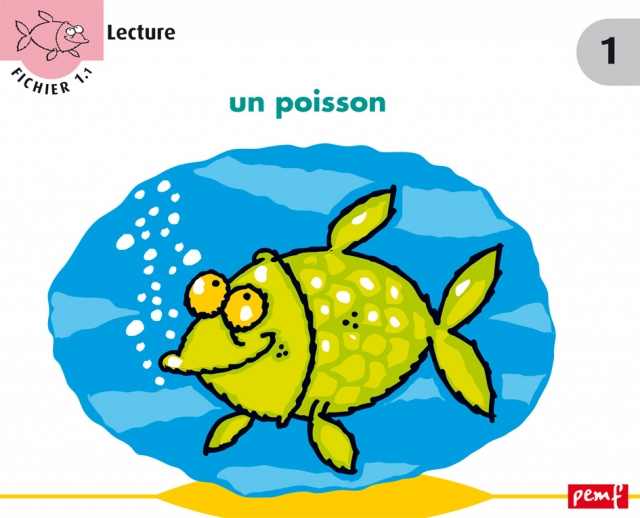
\includegraphics[width=7cm]{img/GSCP_f1recto.jpg}
   \end{minipage}  
   \begin{minipage}[c]{.46\linewidth}
      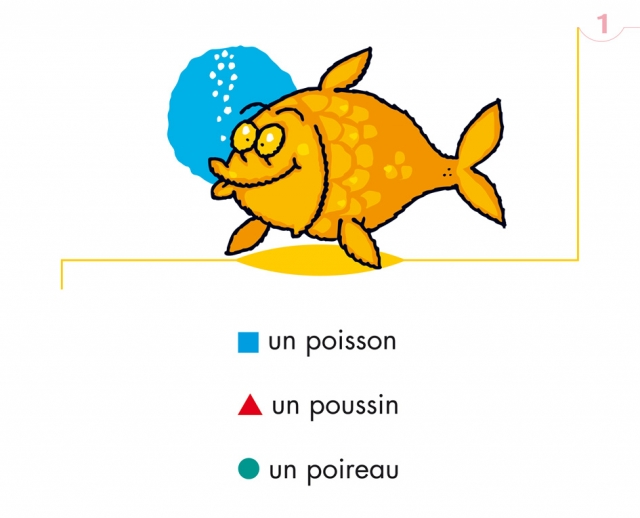
\includegraphics[width=7cm]{img/GSCP_f1verso.jpg}
   \end{minipage}
\end{figure}
\vline
\vline
\begin{figure}[h]
   \begin{minipage}[c]{.46\linewidth}
      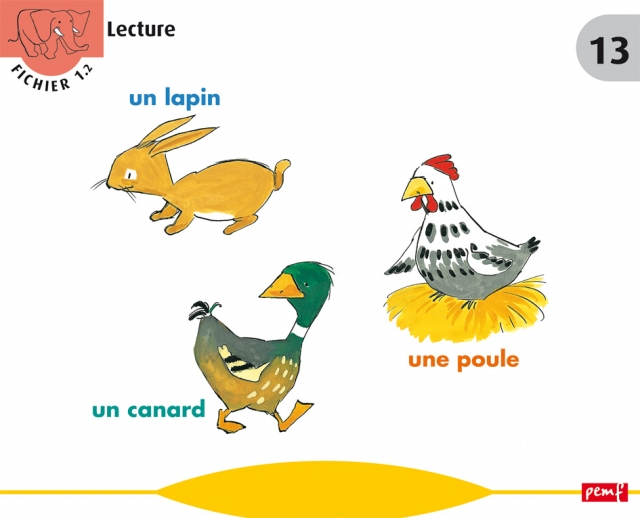
\includegraphics[width=7cm]{img/CP_niv2_f13recto.jpg}
   \end{minipage}  
   \begin{minipage}[c]{.46\linewidth}
      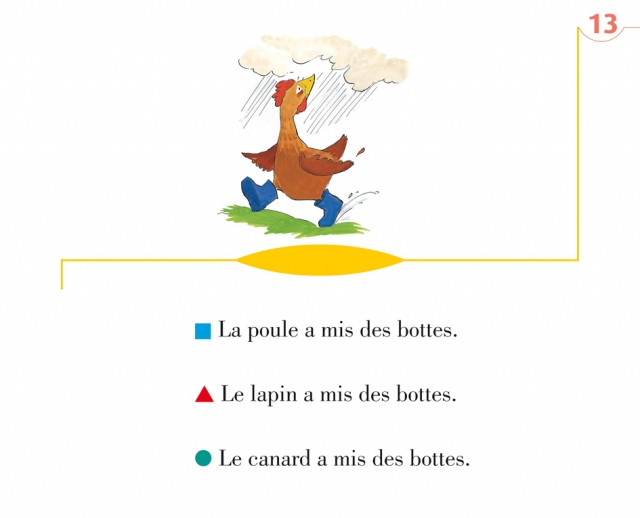
\includegraphics[width=7cm]{img/CP_niv2_f13verso.jpg}
   \end{minipage}
\end{figure}
\vline
\vline
\begin{figure}[h]
   \begin{minipage}[c]{.46\linewidth}
      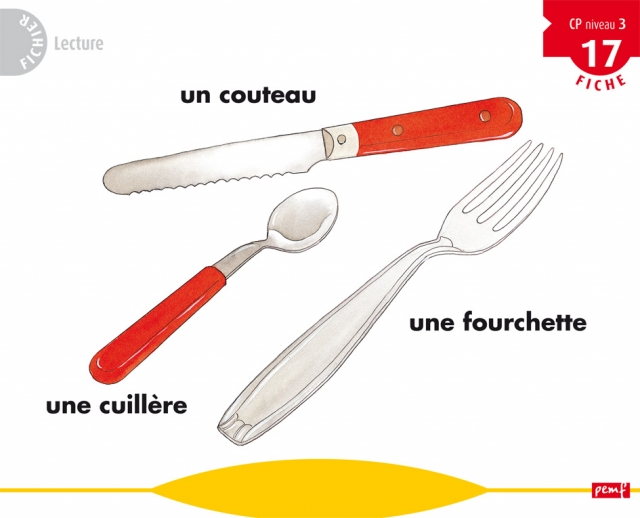
\includegraphics[width=7cm]{img/CP_niv3_f17recto.jpg}
   \end{minipage}  
   \begin{minipage}[c]{.46\linewidth}
      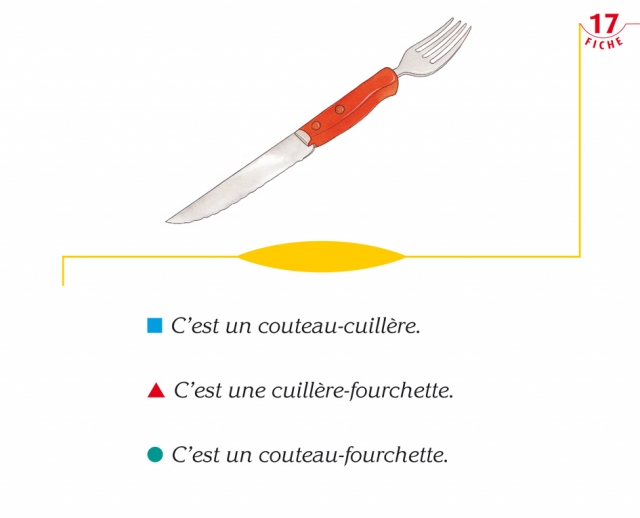
\includegraphics[width=7cm]{img/CP_niv3_f17verso.jpg}
   \end{minipage}
\end{figure}
\end{center}

